\documentclass[runningheads]{llncs}

% ---------------------------------------------------------------
% Include basic ECCV package
 
% TODO REVIEW: Insert your submission number below by replacing '*****'
% TODO FINAL: Comment out the following line for the camera-ready version
\usepackage[review,year=2026,ID=15]{eccv}
% TODO FINAL: Un-comment the following line for the camera-ready version
%\usepackage{eccv}

% OPTIONAL: Un-comment the following line for a version which is easier to read
% on small portrait-orientation screens (e.g., mobile phones, or beside other windows)
%\usepackage[mobile]{eccv}


% ---------------------------------------------------------------
% Other packages

% Commonly used abbreviations (\eg, \ie, \etc, \cf, \etal, etc.)
\usepackage{eccvabbrv}

% Include other packages here, before hyperref.
\usepackage{graphicx}
\usepackage{booktabs}

% The "axessiblity" package can be found at: https://ctan.org/pkg/axessibility?lang=en
\usepackage[accsupp]{axessibility}  % Improves PDF readability for those with disabilities.


% ---------------------------------------------------------------
% Hyperref package

% It is strongly recommended to use hyperref, especially for the review version.
% Please disable hyperref *only* if you encounter grave issues.
% hyperref with option pagebackref eases the reviewers' job, but should be disabled for the final version.
%
% If you comment hyperref and then uncomment it, you should delete
% main.aux before re-running LaTeX.
% (Or just hit 'q' on the first LaTeX run, let it finish, and you
%  should be clear).

% TODO FINAL: Comment out the following line for the camera-ready version
%\usepackage[pagebackref,breaklinks,colorlinks,citecolor=eccvblue]{hyperref}
% TODO FINAL: Un-comment the following line for the camera-ready version
\usepackage{hyperref}
\usepackage{lipsum}
\usepackage{booktabs}
% Support for ORCID icon
\usepackage{orcidlink}

\usepackage{hyperref}
\usepackage{url}

\usepackage{colortbl}
\usepackage{xcolor}
\usepackage{multirow}
\usepackage{subcaption}
\usepackage{amssymb}
\usepackage{pifont}
\usepackage{blindtext}
\usepackage{array}
\usepackage{cellspace}
\usepackage[utf8]{inputenc}
\usepackage{algorithm}
\usepackage{algpseudocode}
\usepackage{amsmath}
\usepackage{amssymb}
\usepackage{booktabs} % for better tables
\usepackage{array} % for better column formatting
\usepackage{pifont}
\usepackage{array}
\usepackage{mwe}

\usepackage[table]{xcolor}
\usepackage{colortbl}
\usepackage{graphicx}
\usepackage{booktabs}
\usepackage{multirow}
\usepackage{wrapfig} 

% -----------------------------사용자 정의 함수----------------------------------
\usepackage{xcolor} % 색상 패키지 불러오기
\definecolor{mygreen}{RGB}{0, 128, 0}
\newcommand{\good}[1]{\textcolor{mygreen}{(#1)}} % 테이블용
\newcommand{\bad}[1]{\textcolor{red}{(#1)}}



\begin{document}

% ---------------------------------------------------------------
% TODO REVIEW: Replace with your title
\title{UMM Transferability} 

% TODO REVIEW: If the paper title is too long for the running head, you can set
% an abbreviated paper title here. If not, comment out.
\titlerunning{Abbreviated paper title}

% TODO FINAL: Replace with your author list. 
% Include the authors' OCRID for the camera-ready version, if at all possible.
\author{First Author\inst{1}\orcidlink{0000-1111-2222-3333} \and
Second Author\inst{2,3}\orcidlink{1111-2222-3333-4444} \and
Third Author\inst{3}\orcidlink{2222--3333-4444-5555}}

% TODO FINAL: Replace with an abbreviated list of authors.
\authorrunning{F.~Author et al.}
% First names are abbreviated in the running head.
% If there are more than two authors, 'et al.' is used.

% TODO FINAL: Replace with your institution list.
\institute{Princeton University, Princeton NJ 08544, USA \and
Springer Heidelberg, Tiergartenstr.~17, 69121 Heidelberg, Germany
\email{lncs@springer.com}\\
\url{http://www.springer.com/gp/computer-science/lncs} \and
ABC Institute, Rupert-Karls-University Heidelberg, Heidelberg, Germany\\
\email{\{abc,lncs\}@uni-heidelberg.de}}

\maketitle


\begin{abstract}
Unified Multimodal Models (UMMs) that jointly handle visual understanding and generation within a single framework have gained significant attention. However, whether and how these two tasks mutually benefit each other through shared representations remains underexplored. In this work, we investigate bidirectional task transferability between understanding and generation in UMMs. Through systematic experiments—comparing joint training against single-task baselines and evaluating Und→Gen and Gen→Und transfer scenarios—we demonstrate that both directions exhibit positive transfer: understanding pretraining provides semantic priors that improve generation quality, while generation training enhances fine-grained visual representations that benefit understanding performance. Our findings suggest that understanding and generation are not competing objectives but complementary ones, and that representational bottlenecks, rather than inherent task conflicts, have been the primary obstacle to realizing their synergy in unified models.
  \keywords{First keyword \and Second keyword \and Third keyword}
\end{abstract}

\section{Introduction}

Multimodal Large Language Models (MLLMs) and diffusion-based generative models~\cite{} have each achieved remarkable progress in recent years. Despite their respective successes, these two model families have evolved largely in isolation: one focuses on interpreting the visual world, and the other on generating it. This naturally motivates the constrcution of a unified model capable of jointly performing understanding and generation. In response, recent Recent Unified Multimodal Models (UMMs)~\cite{} have emerged as a early attempts to integrate these capabilities within a single architecture, achieving performance comparable to expert models in each domain. However, this progress leads to a fundamental inquiry: is the goal of UMMs simply to consolidate two expert systems into one parameter space, or to achieve genuine synergy between understanding and generation that enables a deeper form of world modeling?

% To address this question, we must first determine whether meaningful synergy actually emerges within UMMs. 
Several prior works suggest that complementarity between perception and generation is possible. For example, REPA improves diffusion generation by aligning intermediate DiT representations with DINOv2 features, and other works have shown that auxiliary reconstruction objectives can enhance visual understanding in MLLMs. However, it remains unclear whether such synergy naturally arises within unified architectures. While some studies report positive interactions between tasks, others observe interference, where joint modeling degrades performance. We argue that this discrepancy stems from how synergy has been evaluated. Existing approaches typically rely on aggregate performance changes on general multimodal benchmarks, which do not directly measure whether knowledge learned in one task influences the representations used for another. True synergy cannot be reduced to parameter sharing; it requires knowledge integration, where knowledge acquired from one task meaningfully shapes the representations underlying the other. Therefore, evaluating synergy in UMMs demands a more direct measurement of cross-task knowledge transfer.

To this end, we propose task transferability as a concrete indicator of knowledge integration. Specifically, we examine whether learning in one modality, understanding or generation, can directly improve performance in the other without explicit supervision in that target modality.  As a testbed, we focus on counting, a capability known to be challenging for both MLLMs and diffusion models. We measure whether counting-focused visual instruction tuning improves counting-aware image generation, and conversely, whether counting-aware generative training enhances counting performance in understanding. Through systematic experiments across representative UMM architectures, we find a clear architectural distinction between models that exhibit bi-directional transferability and those that do not. Transferability consistently emerges only in architectures equipped with a shared transformer backbone and a unified image tokenizer. In contrast, loosely coupled designs fail to demonstrate meaningful cross-modal improvement. These findings suggest that knowledge integration is not an automatic consequence of joint training, but is fundamentally shaped by architectural design, highlighting the importance of structural coupling for enabling synergy.

Finally, we extend our analysis beyond counting to investigate how transferability manifests across tasks of varying granularity. From fine-grained tasks such as OCR to coarse semantic reasoning such as spatial position estimation, we observe that different tasks exhibit modality preference—some are more effectively learned through understanding and then transferred to generation, while others benefit from the reverse direction. Notably, in several cases, training in the modality more naturally aligned with a task and subsequently transferring to the target modality yields greater efficiency than direct supervision in the target itself. These findings reveal that the relationship between understanding and generation is neither trivial nor symmetric, but depends on both task characteristics and architectural structure. Our study thus reframes UMM design not as simple functional unification, but as the deliberate construction of architectures capable of genuine knowledge integration

Our contributions ar as follows:
\begin{itemize}
    \item first
    \item second
    \item third
\end{itemize}
\section{Related Work}
\subsection{Unified Multimodal Model}
% 모델 아키텍쳐 위주로
\lipsum[1]
\subsection{Discussions on the synergy between generation and understanding in UMMs}
% ablation study / benchmark 위주의 분석
\lipsum[1]

\section{Does knowledge transfer emerge in UMMs?}
\label{sec:umms}

\begin{figure*}[t]
    \centering
    \includegraphics[width=\linewidth, height=0.25\textheight]{example-image-duck} 
    \vspace{-5pt}
    \caption{TBD, categorize umm archs}
    \label{fig:arch_categorize}
    \vspace{-5pt}
\end{figure*}

Following the architectural taxonomy shown in Figure~\ref{fig:arch_categorize}, we select one representative model from each category for the experiments in this section: (a) Bagel~\cite{deng2025bagel}, (b) Janus-Pro~\cite{chen2025januspro}, (c) Lumina-DiMOO~\cite{xin2025lumina}, and (d) BLIP3-o~\cite{chen2505blip3}.
\subsection{(toy exp)}

\begin{figure*}[t]
    \centering
    \includegraphics[width=\linewidth, height=0.3\textheight]{example-image-duck} 
    \vspace{-5pt}
    \caption{TBD, toy experiment}
    \label{fig:toy_exp}
    \vspace{-5pt}
\end{figure*}

\begin{itemize}
    \item Toy experiments: Train an arbitrary character via text-based instruction tuning (for understanding), and examine whether the generation reflects the learned attributes.
    \item Generation prompt: ``a photo of the man named Samuel''
\end{itemize}


\subsection{(Task transferability across different models)}
% 모델 selct 어떻게 했는지
\begin{table*}[t]
\centering
\begin{tabular*}{\textwidth}{@{\extracolsep{\fill}}cc|cccccccc}
\toprule
\multirow{2}{*}{\textbf{Train}} 
& \multirow{2}{*}{\textbf{Test}} 
& \multicolumn{2}{c}{\textbf{Bagel}} 
& \multicolumn{2}{c}{\textbf{Janus-pro}} 
& \multicolumn{2}{c}{\textbf{Lumina}} 
& \multicolumn{2}{c}{\textbf{Blip3o}} \\

& & Acc. & MAD 
  & Acc. & MAD 
  & Acc. & MAD 
  & Acc. & MAD \\
\midrule

\multirow{2}{*}{Baseline} 
& Und. &  &  &  &  &  &  &  &  \\
& Gen. &  &  &  &  &  &  &  &  \\
\midrule


\multirow{2}{*}{Und.} 
& Und. &  &  &  &  &  &  &  &  \\
& Gen. &  &  &  &  &  &  &  &  \\
\midrule

\multirow{2}{*}{Gen.} 
& Und. &  &  &  &  &  &  &  &  \\
& Gen. &  &  &  &  &  &  &  &  \\

\bottomrule
\end{tabular*}
\caption{Transferability across different models}
\label{tab:transfer}
\end{table*}

To more systematically quantify the observations from Section~\ref{}, we move to a task-level analysis. Specifically, we design experiments around quantity-aware reasoning, which manifests as object \textbf{counting} on the understanding side and \textbf{count-conditioned generation} on the generation side. Since both tasks share the same underlying concept of object quantity, they provide a common evaluation axis for directly measuring whether numerical knowledge learned from one objective transfers to the other. To verify the directionality of this transfer, we set up two complementary training conditions: training with only the understanding objective and evaluating generation performance (Und. $\rightarrow$ Gen.), and vice versa (Gen. $\rightarrow$ Und.).

\subsubsection{Experimental setting.} For training, we filter the PixMo-Points~\cite{deitke2025molmo} dataset to retain samples with object counts ranging from 0 to 20 and reformulate them as counting-based visual instruction tuning data. We further construct generation training data from the same images by employing Qwen3-VL~\cite{bai2025qwen3} to produce image descriptions and explicitly appending object count information as generation prompts. For evaluation, we prepare two separate protocols. Understanding is evaluated on the test split of the PixMo-Count~\cite{deitke2025molmo} dataset. In terms of generation, we follow the counting evaluation protocol from GenEval~\cite{ghosh2023geneval}. We construct generation prompts in the form \mbox{\texttt{"A photo of [NUMBER] [OBJECT]s"}} with object counts ranging from 2 to 10. Generated images are then evaluated using an object detector~\cite{cheng2022masked} to verify whether the number of detected objects matches the specified count. We report both accuracy and mean absolute deviation (MAD) to measure not only exact correctness but also how close predictions are to the ground truth. 

\subsubsection{(Transferability)} Table~\ref{tab:transfer} summarizes the results of the quantity-aware reasoning experiments. For Janus-Pro~\cite{chen2025januspro} and Blip3-o~\cite{chen2505blip3}, training with only one objective does not lead to noticeable gains on the opposite task compared to the baseline. In contrast, BAGEL~\cite{deng2025bagel} and Lumina-DiMOO~\cite{xin2025lumina} show a clear pattern of bi-directional knowledge transfer. Models trained solely with the understanding objective achieve higher accuracy and lower MAD on count-conditioned generation, indicating that the model acquires more precise numerical concepts. Conversely, training only with the generation objective also improves object counting on the understanding side. This suggests that the numerical concept acquired through one objective generalizes to the other. 
It is worth noting that among the four models, Lumina-DiMOO~\cite{xin2025lumina} exhibits the strongest transferability. Remarkably, training Lumina-DiMOO~\cite{xin2025lumina} with only the understanding objective yields even greater improvement in generation performance than directly training on the generation task itself, suggesting that cross-task transfer can serve as a more effective learning signal than direct supervision in this setting.

% \subsubsection{(Disucssion)}From an architectural perspective, Lumina-DiMOO~\cite{xin2025lumina}, which corresponds to category (c) in Figure~\ref{}, employs a shared transformer backbone in which understanding and generation operate on the same image representation. 
% Since understanding and generation reference the identical representation space, any update from one objective is immediately visible to the other, enabling knowledge sharing without requiring a separate bridge or alignment module. 
% This observation aligns with recent studies~\cite{wu2025harmonizing, jiao2025unitoken, wu2026liquid} that advocate for a unified visual representation to promote mutual benefit between understanding and generation, and provides empirical evidence that the degree of representation sharing is a critical factor in enabling cross-task transfer.

\section{Transferability to extended tasks}
The experiments in Section~\ref{sec:umms} established that knowledge transfer between understanding and generation occurs in UMMs with certain architectural properties, and that for counting, this transfer is bi-directional. A natural follow-up question is whether similar patterns hold for other tasks. We investigate this by extending our analysis to two additional domains: OCR, where understanding and generation share character-level visual patterns, and spatial reasoning, where both tasks rely on relative object locations. Throughout this section, we use Lumina-DiMOO~\cite{xin2025lumina} with LoRA-based supervised fine-tuning, as it exhibited the strongest cross-task transfer in the preceding experiments.

\subsection{Text recognition and generation}
We first examine text recognition~(OCR) and text-contained image generation as a pair of complementary tasks. Both tasks operate on character-level visual cues such as strokes, spacing, and glyph structure, requiring the model to capture highly localized and fine-grained visual details. We investigate whether learning such details through one objective transfers to the other.

% \begin{figure*}[t]
%     \centering
%     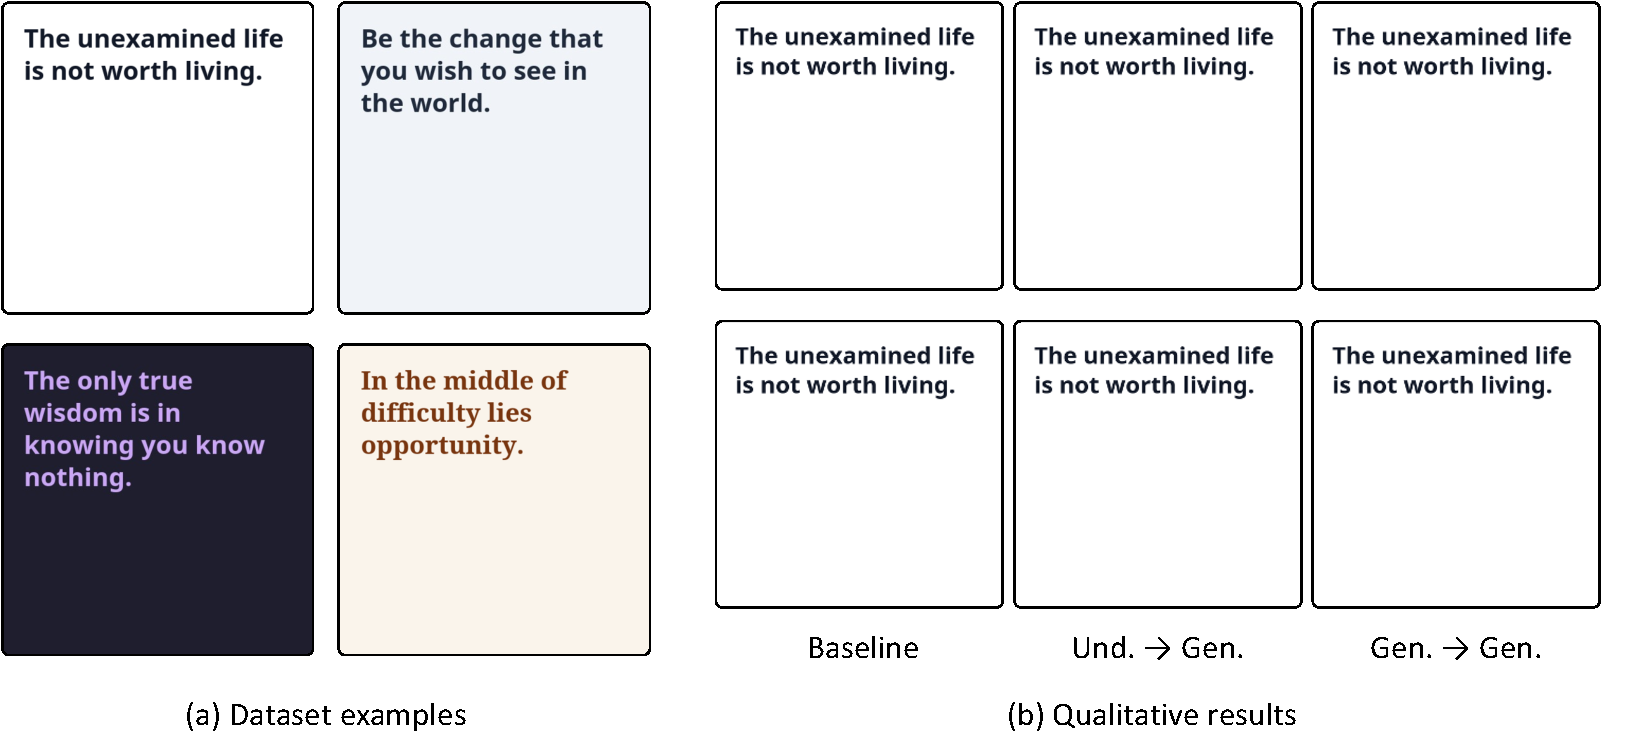
\includegraphics[width=\linewidth]{fig/files/ocr_data_qual.pdf} 
% \caption{(a) Examples from our synthetically rendered Markdown dataset used for both text recognition and text generation training. (b) Qualitative results of text-conditioned image generation under three conditions: Baseline (no fine-tuning), Und.$\rightarrow$
% Gen. (trained only on text recognition), and Gen.$\rightarrow$Gen. (trained and evaluated on text generation).}  
% \label{fig:ocr_data_qual}
% \end{figure*}
\begin{wrapfigure}[15]{r}{0.33\linewidth}
    \centering
    \vspace{-20pt}
    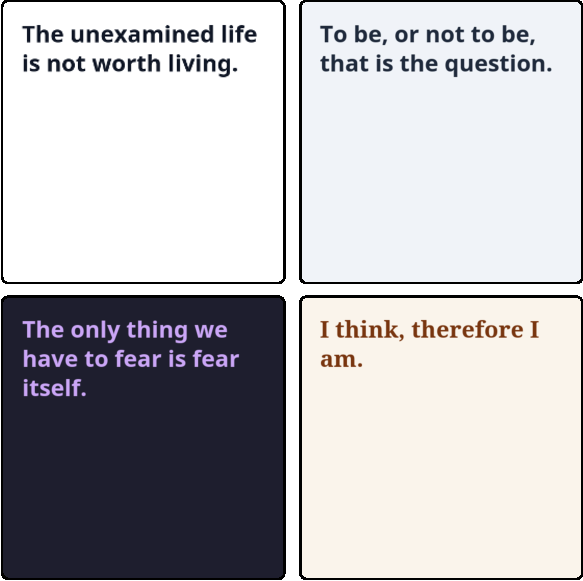
\includegraphics[width=\linewidth]{fig/files/ocr_dataset.pdf}
    \vspace{-5pt}
    \caption{\textbf{Dataset for text recognition and generation.} }
    \label{fig:ocr_dataset}
    \vspace{-40pt}
    \end{wrapfigure}

\subsubsection{Experimental setting.} We construct a dataset of 200K image-text pairs by rendering Markdown documents into images. Existing OCR benchmarks~\cite{} tend to focus on either short sign-level text in natural scenes or dense full-page documents. Neither setting allows meaningful variation in both recognition and generation. Our rendered dataset provides diverse text content at a moderate difficulty level where both tasks can exhibit measurable room for improvement. 
For evaluation, We report five metrics. word error rate (WER) and character error rate (CER) measure exact correctness at the word and character level. Edit Distance captures the minimum number of operations needed to align the prediction with the ground truth. METEOR~\cite{banerjee2005meteor} and F1 assess partial matches by accounting for token overlap and ordering. For understanding, these metrics are computed between the model's output and the ground-truth text. For generation, we first apply an OCR model~\cite{glmocr} to read text from the generated image and then compute the same metrics against the original prompt.
\begin{table*}[!t]
\centering
\begin{tabular*}{\textwidth}{@{\extracolsep{\fill}}cc|cccccc}
\toprule
\multicolumn{2}{c|}{\textbf{Train $\rightarrow$ Test}} 
& \textbf{WER}
& \textbf{CER}
& \textbf{Edit Dist.}
& \textbf{BLEU}
& \textbf{METEOR}
& \textbf{F1}
\\
\midrule

\multirow{2}{*}{Baseline} 
& Und. &  &  &  &  &  &   \\
& Gen. &  &  &  &  &  &   \\
\midrule

\multicolumn{2}{c|}{Und. $\rightarrow$ Und.} &  &  &  &  &  &  \\
\multicolumn{2}{c|}{Und. $\rightarrow$ Gen.} &  &  &  &  &  &  \\
\midrule
\multicolumn{2}{c|}{Gen. $\rightarrow$ Und.} &  &  &  &  &  &  \\
\multicolumn{2}{c|}{Gen. $\rightarrow$ Gen.} &  &  &  &  &  &  \\
\bottomrule
\end{tabular*}
\caption{OCR results of Lumina}
\label{tab:transfer}
\end{table*}

\subsubsection{Generation training improves recognition but not the reverse.} Table~\ref{tab:ocr} summarizes the OCR transfer results. A clear asymmetry emerges between the two transfer directions. Training with the generation objective alone leads to consistent improvement in OCR accuracy across models (\textit{gen}\ $\rightarrow$ \textit{und}). In contrast, training with the understanding objective yields limited gains in text rendering quality (\textit{und}\ $\rightarrow$ \textit{gen}). We attribute this asymmetry to the nature of the two tasks. This contrasts with the counting results in Section~\ref{sec:umms}, where bi-directional transfer was observed.

\subsection{Spatial relation}
\label{sec:spatial_rel}
The previous experiments focus on fine-grained visual details at the character level. We now shift to spatial position, where the model must reason about the coarse layout of objects in a scene. Unlike OCR, spatial reasoning requires understanding semantic relationships between objects rather than local visual patterns. We ask whether learning to recognize spatial arrangements transfers to generating them, and vice versa.

\begin{figure*}[t]
    \centering
    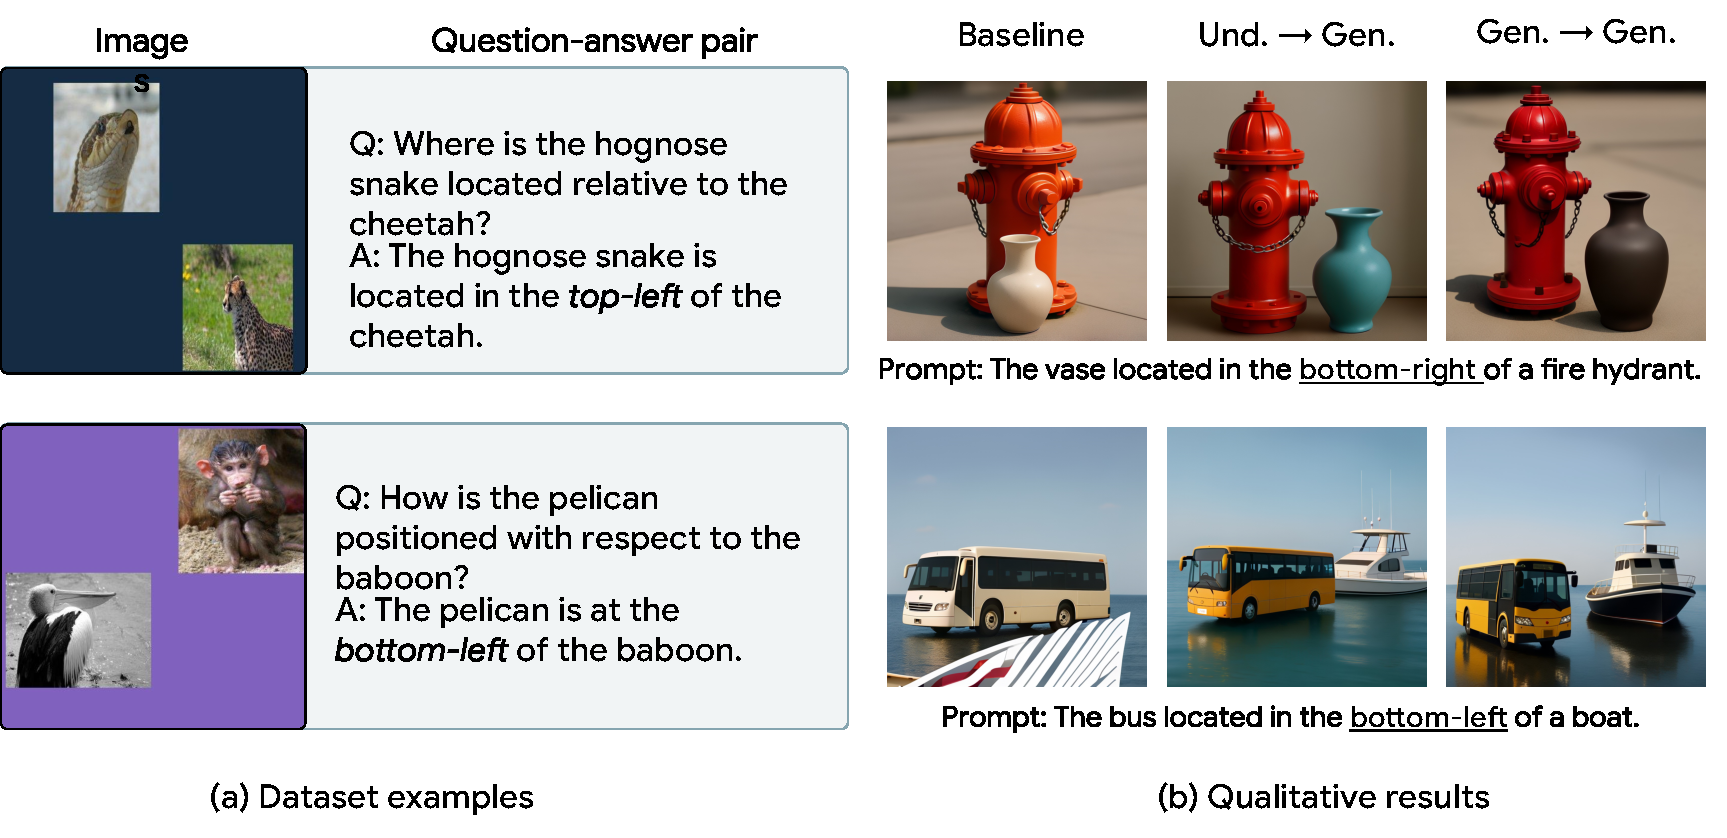
\includegraphics[width=\linewidth]{fig/files/spatial_relation_v2.pdf} 
    \vspace{-5pt}
    \caption{TBD, spatial position}
    \label{fig:spatial_pos}
    \vspace{-5pt}
\end{figure*}


\subsubsection{Experimental setting.} The pre-trained models already handle simple spatial relations such as left, right, top, and bottom reasonably well. We therefore focus on a more challenging setting: diagonal relations between two objects (e.g., top-left, top-right, bottom-right, bottom-left). Since existing spatial reasoning datasets~\cite{} lack the scale and complexity needed for fine-tuning, we construct a synthetic dataset of 200K samples from ImageNet~\cite{}. For each sample, we select two class-image pairs and place them on a canvas according to a randomly sampled diagonal direction. Each sample is paired with a prompt of the form \texttt{"[class A] is located in the [direction] of [class B]"}.
\begin{wraptable}{r}{0.4\textwidth}
    \centering
    \vspace{-20pt}
    \resizebox{0.33\textwidth}{!}{%
        \begin{tabular}{c|c}
            \toprule
            \textbf{Train} 
            & \textbf{Acc.}~$\uparrow$
            \\
            \midrule
            \rowcolor{gray!15}
            \multicolumn{2}{l}{\textit{Understanding}} \\
            Baseline 
            & 0.61 \\
            Und. $\rightarrow$ Und.
            & 0.89 \good{+0.28} \\
            Gen. $\rightarrow$ Und.
            & 0.67 \good{+0.06} \\
            \midrule
            \rowcolor{gray!15}
            \multicolumn{2}{l}{\textit{Generation}} \\
            Baseline
            & 0.67 \\
            Und. $\rightarrow$ Gen.
            & 0.74 \good{+0.07} \\
            Gen. $\rightarrow$ Gen.
            & 0.80 \good{+0.13} \\
            \bottomrule
        \end{tabular}
    }
    \caption{}
    \label{tab:spatial_position_transfer}
    \vspace{-20pt}
\end{wraptable}
For evaluation, understanding is assessed by presenting images in the same format and asking the model to select the correct direction from multiple choices. For generation, we construct prompts in the same format as the training data. Following GenEval~\cite{ghosh2023geneval}, generated images are evaluated by applying a detection model~\cite{} to localize bounding boxes of the two objects. We compute the center points of the detected boxes and verify whether their relative position matches the specified direction.

\subsubsection{Spatial knowledge transfers bi-directionally.} 
Figure~\ref{fig:spatial_pos} summarizes the results. Training with the understanding objective alone improves generation accuracy. Training with the generation objective alone similarly improves understanding. The magnitude of transfer is comparable in both directions. This pattern is consistent with the quantity-aware reasoning results in Section~\ref{sec:umms} and contrasts with the asymmetric transfer observed in text recognition and generation.

\section{Discussion}
\subsection{(what determines transferability?)}

Taken together, our results across three tasks suggest that both the direction and the strength of transfer depend on the nature of the visual attributes a model must internalize to solve each task.


For counting and spatial relations, the key attributes are coarse semantic signals such as object numerosity and layout. These signals tend to be encoded at a similar level regardless of whether the model is trained with an understanding-oriented or generation-oriented objective. Notably, the semantic representations learned through understanding can also provide effective guidance for generation. This observation aligns with prior work showing that improving semantic representations can directly benefit generative performance~\cite{yu2024repa, zheng2025rae}. In our experiments, a model trained to understand counting develops representations that reliably capture the number of objects in an image, and these representations remain useful when the model is asked to generate images containing a specified number of objects. Similarly, training for spatial-relation understanding encourages representations that encode relative object configurations, which can be exploited during generation to produce the intended layout. In other words, semantic knowledge acquired through understanding can meaningfully condition the generation process. When the shared concept is sufficiently coarse and can be captured at a semantic level, this conditioning effect can operate in both directions, leading to bi-directional transfer.

In contrast, text recognition and text generation exhibit an asymmetric transfer pattern. A generation objective requires the model to synthesize individual characters with pixel-level fidelity, and the resulting fine-grained character representations transfer naturally to recognition. The reverse direction is comparatively weaker. While prior studies report that recognition training can facilitate text generation~\cite{ji2023improving, fang2025recognsyn, min2025tair}, we also observe only limited transfer from understanding to generation in this setting. A plausible explanation is that recognition-oriented training primarily emphasizes high-level textual content and identity, whereas text generation additionally demands low-level, spatially precise rendering details. Consequently, semantic knowledge extracted from recognition alone is insufficient to fully bridge the gap to pixel-accurate character synthesis. Overall, our findings indicate that when the shared concept requires fine-grained, pixel-level precision, semantic representations from understanding provide only partial support for generation.

\subsection{}
% transferability 의 application potential




% ---- Bibliography ----
%
% BibTeX users should specify bibliography style 'splncs04'.
% References will then be sorted and formatted in the correct style.
%
\bibliographystyle{splncs04}
\bibliography{main}
\end{document}
